\documentclass[10pt,a4paper]{article}
\usepackage[utf8]{inputenc}
\usepackage[german]{babel}
\usepackage{mathrsfs}
\usepackage{amsmath}
\usepackage{amsfonts}
\usepackage{amssymb}
\usepackage{amsthm}
\usepackage[left=2cm,right=2cm,top=2cm,bottom=2cm]{geometry}
\usepackage{graphicx}
\usepackage{minted}
\usepackage{ulem}

\begin{document}

\section{Aufgabe 1}

\subsection{Teil a}

Let $i, j \in \{ 1, \dots, n \}$.
\begin{align*}
  H_{ij} & = I_{ij} - \frac{1}{n} 1_{n,i}1_{n,j}\\
         & = I_{ij} - \frac{1}{n} \cdot 1\\
         & = I_{ji} - \frac{1}{n} 1_{n,j}1_{n,i}\\
         & = H_{ji}
\end{align*}

\subsection{Teil b}

Let $i, j \in \{ 1, \dots, n \}$.
\begin{align*}
  (HH)_{ij} & = \sum_{k = 1}^{n} H_{i, k}H_{k, j}\\
            & = \sum_{k = 1}^{n} \left( I_{i, k} - \frac{1}{n} 1_{n, i}1_{n, k} \right)\left( I_{k, j} - \frac{1}{n} 1_{n, k}1_{n, j} \right)\\
            & = \sum_{k = 1}^{n} \left( I_{i, k} - \frac{1}{n} \right)\left( I_{k, j} - \frac{1}{n} \right)\\
            & = \sum_{k = 1}^{n} I_{i, k}I_{k, j} - \frac{1}{n} I_{i, k} - \frac{1}{n} I_{k, j} + \frac{1}{n^{2}} \\
            & = [i = j] - \frac{1}{n}I_{ii} - \frac{1}{n} I_{jj} + n \cdot \frac{1}{n^{2}}\\
            & = [i = j] - \frac{1}{n}\\
            & = I_{ij} - \frac{1}{n}\\
            & = I_{ij} - \frac{1}{n} 1_{n,i}1_{n,j}\\
            & = H_{ij}
\end{align*}
Furthermore is $H$ square, so $HH$ is of the same size as $H$. This, in
combination with the fact $(HH)_{ij} = H_{ij}$, proofs, that $H = HH$.

\subsection{Teil c}

Let $i \in \{ 1, \dots, n \}$.
\begin{align*}
  (H1_{n})_{i} & = \sum_{k = 1}^{n} H_{ik}\\
               & = \sum_{k = 1}^{n} I_{ik} - \frac{1}{n} 1_{n,i}1_{n,k}\\
               & = 1 - n \cdot \frac{1}{n} = 0
\end{align*}

\subsection{Teil d}

The eigenvalues are the roots of the characteristic polynomial
\begin{align*}
  \det(\lambda I_{n} - H_{n}) & = \det\left( \lambda I_{n} - I_{n} + \frac{1}{n}\mathbb{O}_{n} \right)
\end{align*}
where $\mathbb{O}_{n}$ is the ones matrix of size $n \times n$. This is $0$, if
the expression in the determinant is not invertible. Besides $\lambda = 0$, this
is also the case for $\lambda = 1$, because all columns of $\mathbb{O}_{n}$ are
linearly dependent. The columns of the inner expression are linearly dependent,
if they can be summed to $0$ with nonzero coefficients. So the following has to
hold for $i \in \{ 1, \dots, n \}$
\begin{align*}
  \xi_{i}\left( \lambda - 1 + \frac{1}{n} \right) + \sum_{j = 1, j \ne i}^{n} \xi_{j}\frac{1}{n} = (\lambda - 1)\xi_{i} + \frac{1}{n} \sum_{j = 1}^{n} \xi_{j} = 0
\end{align*}
If $\lambda = 0$, you can pick the $\xi_{i}$ freely, so that they sum to $0$, so
$0$ is an eigenvalue. If $\lambda = 1$, you get
\begin{equation*}
  \xi_{i} = \frac{1}{n} \sum_{j = 1}^{n} \xi_{j}
\end{equation*}
which can be solved by setting $\xi_{i} = \frac{1}{n}$, so $\lambda = 1$ is
another eigenvalue.

Now suppose $\lambda$ is neither $0$ nor $1$. Then we get
\begin{equation*}
  \xi_{i} = -\frac{1}{\lambda - 1}\frac{1}{n} \sum_{j = 1}^{n} \xi_{j}
\end{equation*}
Adding all $n$ equations, results in
\begin{equation*}
  \sum_{j = 1}^{n} \xi_{j} = -\frac{1}{\lambda - 1} \sum_{j = 1}^{n} \xi_{j} \Leftrightarrow \frac{\lambda}{\lambda - 1} \sum_{j = 1}^{n} \xi_{j} = 0 \Leftrightarrow \sum_{j = 1}^{n} \xi_{j} = 0
\end{equation*}
and plugging this back in the previous equation yields
\begin{equation}
  \xi_{i} = 0 \quad \forall i \in \{ 1, \dots, n \}
\end{equation}
Therefore $\lambda I_{n} - I_{n} + \frac{1}{n}\mathbb{O}_{n}$ is invertible for
all $\lambda$ except $0$ and $1$, so $0$ and $1$ are the only eigenvalues.

\subsection{Teil e}

\begin{align*}
  (XH1_{n})_{i} & = \sum_{k = 1}^{n} \sum_{h = 1}^{n} X_{i,h} H_{h,k}\\
                & = \sum_{k = 1}^{n} \sum_{h = 1}^{n} X_{i,h} \left( I_{h,k} - \frac{1}{n} \right)\\
                & = \sum_{h = 1}^{n} \sum_{k = 1}^{n} X_{i,h} I_{h,k} - \frac{1}{n} X_{i,h}\\
                & = \sum_{h = 1}^{n} X_{i,h} - X_{i,h}\\
                & = \sum_{h = 1}^{n} 0 = 0
\end{align*}

\section{Aufgabe 2}

\subsection{Teil a}

\begin{minted}{julia}
function kpca(X, k; d=size(X,1))
    # inputs:
    #    X       data matrix where each column is a data point, size(X)==(D,n)
    #    k       a kernel function
    #    d       the number of nonlinear directions
    # outputs:
    #    Y       data matrix where is row is a nonlinear direction, size(Y)==(d,n)
    (D, n) = size(X)
    K = float([k(X[:, i], X[:, j]) for i = 1:n, j = 1:n])
    H = eye(n) - (1 / n) * ones(n, n)
    centeredK = H * K * H
    centeredK = (1 / 2) * (centeredK + centeredK') # Symmetrize
    (Lambda, V) = eig(centeredK)
    indices = sortperm(Lambda, rev=true)
    Lambda1 = map(sqrt, Lambda[indices[1:d]])
    V1 = V[:, indices[1:d]]
    Y = diagm(Lambda1) * V1' * centeredK
end
\end{minted}

\subsection{Teil b}

\begin{figure}[h!]
  \centering
  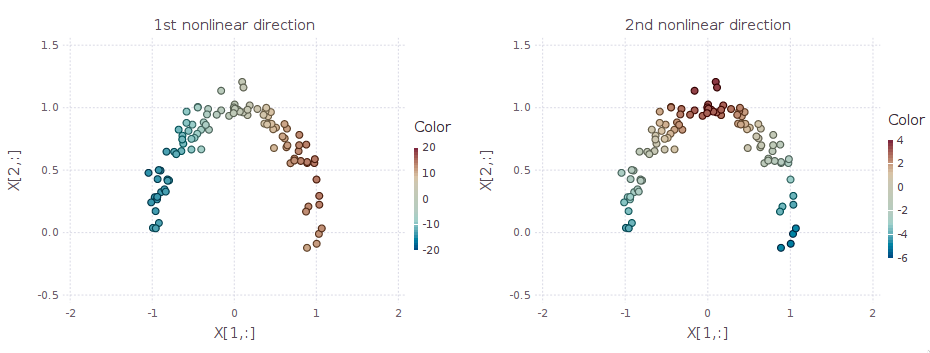
\includegraphics[width=300pt]{7_2_b_1}
  \caption{Toy set \#1}
\end{figure}
To get toy set \#2 to work, you have to delete the line, that permutates the Xs
first. Otherwise the points are not plotted in clusters.
\begin{figure}[h!]
  \centering
  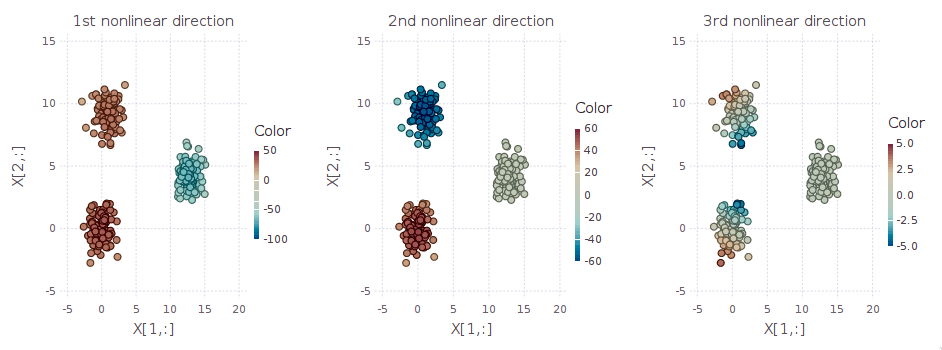
\includegraphics[width=300pt]{7_2_b_2}
  \caption{Toy set \#2}
\end{figure}

\subsection{Teil c}

A two dimensional point along with it's projection onto one of the principal
components represents a point in $\mathbb{R}^{3}$. If the principal components
are linear directions, these points lie on an affine subspace of
$\mathbb{R}^{3}$. So I will try to automatically decide, if a set of components
is linear, by computing a 2D plane via linear regression and then looking at the
mean error over all points.

The function to compute linear regression weights is given by
\begin{minted}{julia}
function linear_regression(X, y)
    (X' * X) \ X' * y
end
\end{minted}
We would like to find a linear (affin) regression, so we transform to an affin
combination.
\begin{minted}{julia}
function Phi(x)
    [1 x[1] x[2]]
end
\end{minted}
The next function computes the mean error from the regression plane over all
points.
\begin{minted}{julia}
function mean_error_from_plane(X, Y)
    # Number of samples
    n = size(X, 1)

    # Transform X
    X2 = vcat([Phi(X[i, :]) for i = 1:n]...)

    # Compute weights
    W = linear_regression(X2, Y)

    # Compute linear approximation to Y
    Y2 = X2 * W

    # Compute error per point
    D = abs(Y - Y2)

    # Compute mean
    ((1 / n) * D' * ones(n, 1))[1, 1] # Extract number from 1x1 matrix
end
\end{minted}
Use the following function to generate ``sheet data''.
\begin{minted}{julia}
function generate_sheet(n, alpha)
    rand(2, n) .* [1, alpha]
end
\end{minted}
And the final function computes the mean errors for the first two directions for
given $\alpha$ and $\sigma$.
\begin{minted}{julia}
function mean_errors(alpha, sigma2)
    X = generate_sheet(1000, alpha)
    k(a, b) = kgauss(a, b, sigma2)
    Y = kpca(X, k, d=3)

    [mean_error_from_plane(X', Y[d, :]') for d = 1:3]
end
\end{minted}
Finally we will compute, how linear the found directions are for a given set of
$\alpha$s and $\sigma^{2}$s.
\begin{minted}{julia}
alphas = 0.5:0.5:10
sigma2s = 0.5:0.5:10
maxErrors = [apply(max, mean_errors(alpha, sigma2)) for alpha = alphas, sigma2 = sigma2s]
\end{minted}
and plot the result
\begin{minted}{julia}
Alphas = hcat([a * ones(1, size(alphas, 1)) for a in alphas]...)
Sigma2s = hcat([sigma2s' for i in 1:size(sigma2s, 1)]...)
Errors = hcat([maxErrors[i, :] for i = 1:size(maxErrors, 1)]...)

plot(x = Alphas, y = Sigma2s, color=Errors,
    Guide.xlabel("alpha"), Guide.ylabel("sigma^2"),
    Guide.colorkey("Mean error"),
    Geom.rectbin)
\end{minted}
\begin{figure}[h]
  \centering
  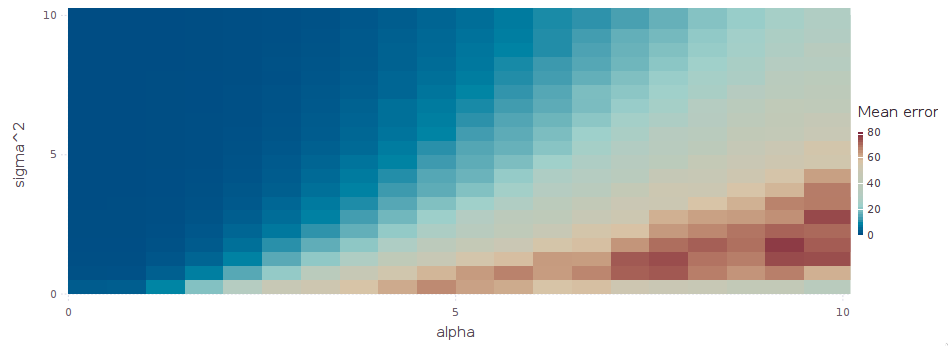
\includegraphics[width=350pt]{7_2_c_graph}
  \caption{How linear are the component directions?}
\end{figure}
Keep in mind, that the numbers are means, so an error of $10$ is already very
non-linear. We can see, that, at least for small parameter values, PCA with the
gauss-kernel selects the linear directions first, if $\sigma^{2} > 2\alpha$.

Let's (kind of) verify, that the graph and numbers tell the truth. We use the
following function to generate the three direction plots, for some given
$\alpha$ and $\sigma^{2}$.
\begin{minted}{latex}
function direction_plots (alpha, sigma2)
    n = 1000
    X = rand(2,n) .* [1, alpha]

    k(a, b) = kgauss(a, b, sigma2)

    Y = kpca(X, k, d=3)

    hstack(plot(x=X[1,:], y=X[2,:], color=Y[1,:],
                Guide.title("1st nonlinear direction"),
                Guide.xlabel("X[1,:]"), Guide.ylabel("X[2,:]")),
           plot(x=X[1,:], y=X[2,:], color=Y[2,:],
                Guide.title("2nd nonlinear direction"),
                Guide.xlabel("X[1,:]"), Guide.ylabel("X[2,:]")),
           plot(x=X[1,:], y=X[2,:], color=Y[3,:],
                Guide.title("3rd nonlinear direction"),
                Guide.xlabel("X[1,:]"), Guide.ylabel("X[2,:]")))
end
\end{minted}
\begin{figure}[ht!]
  \centering
  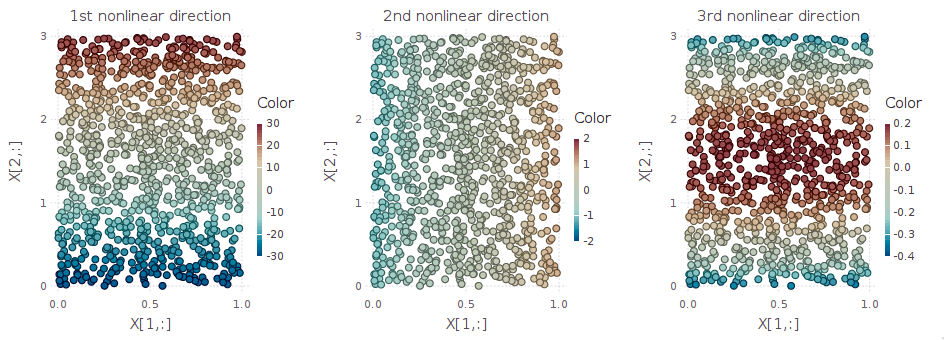
\includegraphics[width=350pt]{7_2_c_linear}
  \caption{\mintinline{julia}{direction_plots(3, 10)}}
\end{figure}
\begin{figure}[ht!]
  \centering
  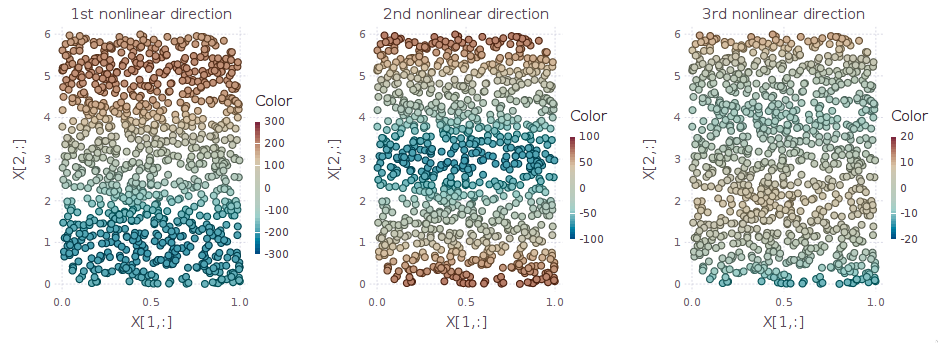
\includegraphics[width=350pt]{7_2_c_nonlinear}
  \caption{\mintinline{julia}{direction_plots(6, 2.5)}}
\end{figure}
You can see, that the directions are linear, if the values are from the deep
blue area, but non-linear otherwise (the second direction is more of a half-pipe
respectively the square of the first direction in the second picture).

\subsection{Teil d}

\sout{
The directions still depend on $\alpha$ because they are found in the order of
decreasing variance. Since the data is arranged in a rectangle with side lengths
$1$ and $\alpha$, the first direction is the direction of the longer side of the
rectangle. If $\alpha > 1$, the first direction is vertical and it is
horizontal, if $\alpha < 1$.}

\sout{
Something interesting happens, when $\alpha = 1$. The data is now arranged in a
square, so the order of directions is no longer predetermined.
}

Ok, strike that. What is actually going on here? We are using the PCA-variant,
that computes all directions at once, so we get the correct solution, but it may
be arbitrarily rotated. But this rotation can only be observed with
$\alpha = 1$. If $\alpha \ne 1$, the directions are sorted as explained above (I
think, I saw a tiny bit of rotation for $\alpha = 5$, but I may be mistaken
here).

Actually the directions are still rotated for $\alpha$s, that are slightly
larger than $1$.
\begin{figure}[ht!]
  \centering
  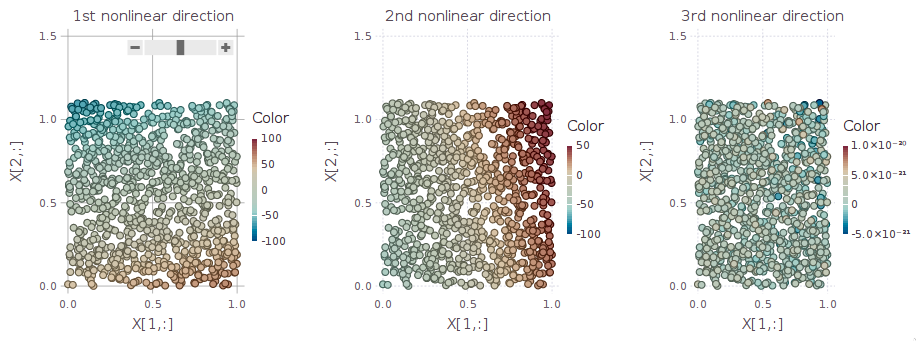
\includegraphics[width=350pt]{7_2_d_rotated}
  \caption{Rotated directions with $\alpha = 1.1$}
\end{figure}
\begin{figure}[ht!]
  \centering
  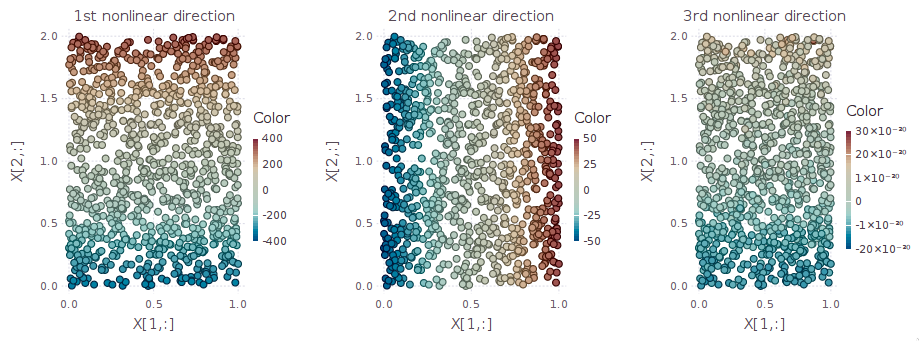
\includegraphics[width=350pt]{7_2_d_straight}
  \caption{Ordered directions for $\alpha = 2$}
\end{figure}

So apparently the answer is, that the directions should not depend on $\alpha$,
but they still do. The directions are always two orthogonal vectors, that span
the $\mathbb{R}^{2}$ and can be arbitrarily rotated. But somehow they are not,
if $\alpha$ is sufficiently far from $1$.

The directions will always be orthogonal for the linear kernel, because they
must be orthogonal in the feature space, but with a linear kernel the feature
space and attribute space are the same.

The directions in b) are orthogonal in the feature space, but that does not
necessitate, that they are orthogonal in 2d.

\end{document}